\section{Data Preparation}
\label{section:data_prepatation}

With a better understanding of the data following its thorough exploration, the final step before modelling begins is to prepare the data. It would possible to include some of the processing of the data described here within the modelling process, for example converting case of all characters to lower case. However, it was decided that performing these steps in advance would allow better control and give greater transparency of the data submitted to classifier models. In this section, the processing or transformations performed are each described before discussing the reasons for each of them.

\subsection{Cleaning the Data}

In total eight transformation steps are applied to the data:

\begin{enumerate}
	\item Convert to lower case
	\item Convert to ASCII
	\item Remove URLs
	\item Remove all punctuation
	\item Replace numeric values 11 to 25 with text values
	\item Remove any digits that remain
	\item Remove any repeating characters
	\item Fix common abbreviations and replace with full word
\end{enumerate}

Python is once again the language of choice to perform these transformations. The data was read from the MySQL database in two blocks, the block of questions that were identified as bullying and the non bullying block. Instead of writing the final questions back to the database the questions were written to a file on disk for later processing by the Python Natural Language Toolkit (NLTK) \cite{bird_natural_2009} as described in Chapter \ref{chapter5}.

The first four transformations are conversion to lower case, the removal of non ASCII characters and URLs and the removal of any remaining punctuation characters. The complete scripts showing the details of how these string manipulations were performed are given in Appendix \ref{app:baseline}. The conversion of all text to lower case is a simple invocation of the \verb|lower| method on the question string which needs no further explanation. During data exploration, it was noticed that there were several characters that were not in the ASCII code set. The \verb|unicodedata.normalize| method shown on lines 28 to 32 of Appendix \ref{app:baseline} will return the normalised version of the passed string. The first parameter passed defines the decomposition to be applied to the Unicode string. Normal form KD (NFKD) will replace all compatibility characters with their equivalents. The string returned is encoded as ASCII. Next a standard regular expression representing a URL is used to remove all URLs by replacing them with an empty string, lines 35 to 38. 

Any remaining punctuation characters are removed next as shown on lines 41 to 45. The \verb|translate| string method takes two arguments. The first is a table of characters to translate, and the second is the list of characters to delete. \verb|string.maketrans| is used to create the table of characters to translate but when used as shown an empty table is created. The list of punctuation characters is passed as the second parameter. The effect of passing an empty table of translation characters and the list of punctuation characters is that the punctuation characters are just deleted which is the desired effect. The sixth transformation uses a slightly differently formatted version of the translate method but is used in the same manner to remove any remaining digits as shown on lines 52 and 53. Rather than passing the punctuation characters in this instance the lists of digits are passed, and \verb|None| represents an empty value in this case an empty table of translation characters.

The other three string manipulation routines replace selected numeric values with text, removes repeating characters and fix an identified number of abbreviations with whole words. From the data exploration, it was noticed that there were a number of bullying questions that requested sensitive personal information such as a persons age. To capture this important information, for use during the modelling process, a new class was developed to allow such a replacement. The details of this class are discussed shortly but the code to execute this substitution is given in lines 48 and 49 of Appendix \ref{app:baseline}. An instance of the \verb|RegexReplacerAge| is created and then the replace method is called on the passed string returning a new string where the required values have been replaced. The \verb|RegexReplacer| class used to replace common word abbreviations uses the same logic taking a string and returning the same string where occurrences of defined abbreviated words are expanded to their full representation.

The final piece of code to be examined is the code that removes repeating characters from the text of the questions. A \verb|RepeatReplacer| object is created as well as any empty array. Then for each word in the question, obtained using the split method, the replace method of the class is called returning a valid word without the repeating characters. The array of words created is then converted back to a string. 

The last three manipulation operations described rely on classes imported from a package in the same folder called \textit{``replacers.py''}. 

\begin{lstlisting}[]
from .replacers import RegexpReplacer
from .replacers import RegexpReplacerAge
from .replacers import RepeatReplacer
\end{lstlisting}

This replacer package is based on a package of the same name described in Python Text Processing with NLTK 2.0 Cookbook (\citet{perkins_python_2010}). The first class to consider is the \verb|RegexpReplacer| class. The core of this class is the \verb|replace()| method which takes a word and returns what is considered a more correct version. Before this class can be utilised an array of replacement patterns, or words, must first be defined. As shown in and Appendix \ref{app:replacer} the first three patterns are used to replace \textit{u} with the full word \textit{you}. For example \verb|(r'(\su\s)', ' you ')| searches the text for any occurrence of the letter u with white space (\verb|\s|) on both sides and replaces this with a space followed by the word ``you'' followed by another space. The two edge cases, where u is the first word in a question or the last word of the question are also handled. The \verb|$| symbol is used to identify the end of the text of the question and the \verb|^| symbol to identify the start of the question. 

The two most important concepts encapsulated in the class are performed by the \verb|re.compile| method and the \verb|re.subn| method. The compile method compiles the regular expression patterns, for example \verb|\su\s|, into a regular expression object. The subn method takes three parameters, the compiled regular expression object, the replacement text value and the string on which to perform the regular expression substitution. The resulting string and the number of substitutions made are returned. 

The \verb|RegexpReplacerAge| class is identical to the \verb|RegexpReplacer| class except that instead of taking text based patterns it is looking to replace digits that are representative of peoples ages. 

Just like the \verb|RegexpReplacer| class, the purpose of the \verb|RepeatReplacer| class, lines 115-130, is to return a more correct version of the word passed for processing. However, instead of replacing abbreviated words with the correct fully expanded word, the goal here is to remove unnecessary repeating characters. This class makes very good use of backreferences to remove these repeating characters. The \verb|repeat_regexp| regular expression will match zero or more characters at the start of the string and these are referenced as \verb|\1|. Next a single character is matched but it must be immediately followed by another instance of itself, referenced as \verb|\2|. Finally zero or more characters at the end of the string and these are referenced as \verb|\3|. Then \verb|repl| simply references \verb|\1 \2 \3| recombined without the single repeated character which is not included as it was not within the grouping parentheses of the second reference. The \verb|replace()| method is then called recursively to remove multiple repeated characters but makes use of a WordNet lookup as a stopping mechanism when a valid word is identified.

\subsection{Write Data in NLTK Corpus Format}

The Python script described in the previous section, shown in Appendix \ref{app:baseline}, was executed separately for questions classified as bullying and for questions classified as not bullying, the SQL on lines 18 and 19 was changed to select each class separately. Processing each class separately in this manner allowed each question to be written individually to a file in a folder named in accordance with the class type, for example bullying questions were written into a folder named \verb|bullying| and not bully question were written to a folder called \verb|not_bullying|. The parent folder for each was called \verb|01| as the dataset produced as a result of this processing will be called \verb|cyberbully_01| in later sections, the original raw data was written to disk in a similar manner without processing to a folder named \verb|00|. The name of the folder that the files were written to, lines 70 and 71, was changed to reflect the class that was being processed. Each question was written to a separate file that was anonymously named in the range \verb|00001| to \verb|99999| so that the question could not be traced back to the original question on the Ask.fm website. 

Once this \verb|01| dataset had been written to disk five further datasets were generated from it. Data \verb|02| and \verb|03| were the bi-grams and tri-grams datasets derived from the original \verb|01| dataset. Next, NLTK stop words were stripped from the \verb|01| dataset producing the \verb|11| dataset from which bi-grams and tri-grams were again generated producing datasets \verb|12| and \verb|13| respectively. The final structure of the NLTK corpora developed here can be seen in Figure \ref{fig:chapter5:corpus_structure}. All dataset manipulation was achieved using Python.

\subsection{Analysis of Cleaning Steps}

It is worth examining some of the changes made to the text of the questions by the processing described here, and explain the relevance of each step.

The conversion of all characters to lower case is a standard step to perform in text mining. The goal is to reduce the number of tokens that will later be presented to the model. For example, whilst the reader understands that \textit{``Why''}, \textit{``WHY''} and \textit{``why''} are all different representations of the same word. If presented to the text mining model in this manner, three distinct tokens will be identified. Interpreting words with different case representations as separate tokens increases the  size of the final word vector and also may have the unwanted side effect of either incorrectly diluting or multiplying the impact of a word in the generation of the classification model. Though capitalisation of words can be used to infer shouting or displeasure, for the purposes of this study it is acceptable that all words are converted to lower case.

Removal of non ASCII characters was performed to clean up the text of the question and remove extra characters added to ``beautify'' the question. It was also to ensure that all text was represented in its simplest form. This processing had the beneficial side effect, like the conversion to lover case, of standardising tokens. Examples of both the removal of unwanted characters and the standardising of text is shown in Figure \ref{fig:chapter4:remove_nonascii}. The first example shows how the non ASCII characters that spelt out the word \verb|beautiful| were converted into normal ASCII characters and the decorative symbols after the word were removed. The second example converted the phrase \verb|Love you Forever| to ASCII as well as removing the heart symbol.

\begin{figure}[htbp]
	\centering
	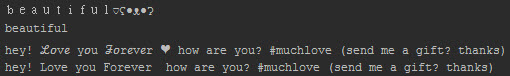
\includegraphics[width=0.85\textwidth]{Figures/Chapter4/remove_nonascii_01.jpg}
	\caption[Remove non ASCII characters]{Samples of where non ASCII characters were either removed or replaced with their ASCII equivalent}
	\label{fig:chapter4:remove_nonascii}
\end{figure}

It was decided that URL strings where so unique that they would not add any significant benefit if included in the model. They were stripped out wherever they were found. The removal of punctuation characters served at least two purposes. The first thing that stripping punctuation characters achieved was to remove all emoticons from the text of the questions. Although it could be argued that the emoticons are representative of the tone or sentiment of the question, it was observed that their use was inconsistent and there were multiple different representations of several emoticons. This all meant that the intended meaning of some emoticons were not obviously clear. In the first two examples shown in Figure \ref{fig:chapter4:remove_punct} it can be seen how removing the punctuation greatly cleans up the presentation of the text. The third examples shows the removal of two emoticons.

\begin{figure}[htbp]
	\centering
	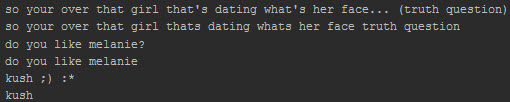
\includegraphics[width=0.85\textwidth]{Figures/Chapter4/remove_punct_01.jpg}
	\caption[Remove punctuation characters]{Samples of where punctuation has been removed showing where emoticons are removed}
	\label{fig:chapter4:remove_punct}
\end{figure}

Next it was decided to remove all numeric characters. However, it was noticed that there were a significant number of references to peoples ages and that most of these related to teenagers or early twenties. This information was considered useful and worth saving so before all other digits were removed the numbers from \textit{``11''} to \textit{``25''} inclusive were replaced with their text equivalent. After these numbers were substituted, all other digits were removed. A sample of an age being replaced with the text value is shown in \ref{fig:chapter4:remove_digit} as well as the removal of all other digits that are deemed not to represent ages.

\begin{figure}[htbp]
	\centering
	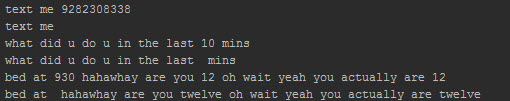
\includegraphics[width=0.9\textwidth]{Figures/Chapter4/remove_digits_01.jpg}
	\caption[Replace selected numerical ages with text then remove remaining digits]{Samples of where certain numbers have be substituted with text values and all other digits are removed}
	\label{fig:chapter4:remove_digit}
\end{figure}

As discussed earlier, the nature of social media means that text is often unstructured. Words are sometimes accentuated with the addition of extra repeated characters or abbreviated to their simplest forms. For example, \textit{``looove yoooou''} or \textit{``love u''} both mean the same thing but if left in this format extra unnecessary tokens will be added to the word vector diluting the effectiveness of the model. Alternatively, shorter tokens will be stripped because they do not meet a minimum token length criterion. In the first case the repeated characters are removed returning a valid word. In the second, a number of abbreviated words and their full text representations were defined. Sample of both these word manipulations can be seen in Figure \ref{fig:chapter4:remove_repeat}. The first two examples show the successful removal of repeated characters whilst the third example shows both repeated characters removed and the replacement of an abbreviated word with the correct word.

\begin{figure}[htbp]
	\centering
	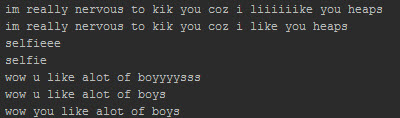
\includegraphics[width=0.75\textwidth]{Figures/Chapter4/remove_repeat_01.jpg}
	\caption[Remove repeated characters and abbreviated words]{Samples of where repeated characters have been removed and abbreviated words are replaced with correct word}
	\label{fig:chapter4:remove_repeat}
\end{figure}


\subsection{Data Exploration Revisited}

Now that \textit{``cleansed''} datasets are available for the not bullying and bullying classes it is worthwhile taking a brief step backwards and analyse these dataset using the same techniques described in Section \ref{section:data_exploration}. For brevity only the not bullying and bullying datasets are considered and only certain measures.

The top ten distinct token frequencies of bi-grams and tri-grams from the bullying dataset is shown in Table \ref{tab:chapter4:word_count_bullying_clean}. Looking first at bi-grams with stop words, eight out of the top ten tokens have not changed but what is noticeable is that overall the frequencies have increased. Looking at the bullying bi-grams with stop words removed only six of the original top ten are still present. Once again the frequencies have increased albeit more modestly. What is significant is that the previous number one most frequently occurring  bi-gram, \verb|right_now|, is now no longer included. Initially it was thought that this was an error, however, upon a more detailed examination it was discovered that the original two tokens were \verb|right| and \verb|now?|. The question mark character prevented \verb|now| from being identified as a stop word. It would appear that the cleaning process has impacted on bullying bi-grams. Whether this impact is positive or negative remains to be seen.

\begin{table}[h]
\centering
\caption[Distinct n-gram word counts (cleaned datasets)]{Table showing distinct counts of bi-gram and tri-gram tokens for the cleaned bullying dataset and also with and without stop words}
\label{tab:chapter4:word_count_bullying_clean}
\begin{tabular}{lrlr}
	\toprule
	\multicolumn{4}{c}{\textbf{Bullying Bi-Grams}} \\
	\cmidrule(r){1-4}
	\multicolumn{2}{c}{\textbf{With Stopwords}} & \multicolumn{2}{c}{\textbf{No Stopwords}} \\
    \midrule
	are\_you	&	155 & post\_pic		& 25	\\
	do\_you		&	106 & dont\_know	& 20	\\
	you\_have	&	65 & wearing\_right	& 20	\\
	you\_are	&	54 & dont\_like		& 13	\\
	of\_you		&	48 & cut\_cut		& 9	\\
	you\_and	&	47 & really\_pretty	& 9	\\
	what\_are	&	44 & post\_selfie	& 8	\\
	if\_you		&	42 & post\_picture	& 8	\\
	how\_old	&	37 & dont\_even		& 8	\\
	would\_you	&	36 & bra\_size		& 7	\\
    \bottomrule
    \end{tabular}
\begin{tabular}{lrlr}
	\toprule
	\multicolumn{4}{c}{\textbf{Bullying Tri-Grams}} \\
	\cmidrule(r){1-4}
	\multicolumn{2}{c}{\textbf{With Stopwords}} & \multicolumn{2}{c}{\textbf{No Stopwords}} \\
    \midrule
	what\_are\_you		& 36 &	cut\_cut\_cut			& 7 \\
	old\_are\_you		& 32 &	last\_person\_kissed	& 5 \\
	how\_old\_are		& 32 &	whoever\_likes\_thinks	& 4 \\
	are\_you\_wearing	& 22 &	see\_window\_post		& 4 \\
	you\_wearing\_right	& 20 &	seem\_really\_nice		& 4 \\
	wearing\_right\_now	& 20 &	window\_post\_pic		& 4 \\
	do\_you\_have		& 17 &	slept\_ex\_bf			& 3 \\
	are\_you\_single	& 17 &	shannon\_slept\_ex		& 3 \\
	of\_you\_and		& 16 &	likes\_thinks\_you're	& 3 \\
	are\_you\_doing		& 14  &	ex\_bf\_max				& 3 \\
    \bottomrule
    \end{tabular}
\end{table}

When the bullying tri-grams that included stop words were re-examined, eight of the top ten remained the same with high count frequencies evident. Surprisingly not only were nine of the top ten tri-grams where stop words had been removed the same as before the dataset was cleaned, but these nine tokens also had the same frequencies. The only token missing from the list was \verb|wearing_right_now| and as previously highlighted with the bi-grams this token is no longer occurring in the list because the genuine stop word \verb|now| is no longer available for consideration. It should be noted that further examination showed that this was not the only such occurrence of where a stop word had not been removed from the dataset because it was attached to a punctuation mark. It was again noticed that where stop words were not removed, personal pronouns were again a very common occurrence in the top ten list.

Table \ref{tab:chapter4:word_distribution_clean} shows the number of unique tokens in each of the cleaned datasets as well as the total count of tokens, and their average frequencies. The numbers in brackets show the percentage increase or decrease when compared with the original data. It is clear to see that nearly all counts are down and that, in general, the average frequencies have either increased or stayed the same. The general decrease in the number of tokens can be explained by the cleaning process where it was seen that many numerical tokens were removed, and multiple variations of the same token were standardised. The slight increase in the number of bullying n-grams with stop words is down to common abbreviations being standardised.

\begin{table}[h]
\centering
\caption[Unique tokens, total count and average frequency (cleaned datasets)]{Table showing the number of distinct tokens in each dataset as well as the total token counts and average frequencies}
\label{tab:chapter4:word_distribution_clean}
\begin{tabular}{lrrl}
	\toprule
	{\textbf{Token}} 		& {\textbf{Unique}} & {\textbf{Total}} & {\textbf{Average}}  \\
	{\textbf{description}}	& {\textbf{Tokens}} & {\textbf{Count}} & {\textbf{Frequency}}  \\
    \midrule
    \midrule
    \multicolumn{1}{l}{\textbf{Not Bullying}} \\
	\cmidrule(l){1-1}
	Uni-Grams					& 6579 (-37\%) &	61293 (-13\%)	& 9.1 (+39\%) \\
	Bi-Grams					& 29149 (-13\%) &	53436 (-13\%)	& 1.8 (same)\\
	Tri-Grams					& 38701 (-5\%) &	46120 (-13\%)	& 1.2 (-8\%) \\
	Uni-Grams No Stop Words		& 6462 (-38\%) &	33156 (-19\%)	& 5.1 (+31\%) \\
	Bi-Grams No Stop Words		& 21172 (-16\%) &	25394 (-20\%)	& 1.2 (-8\%) \\
	Tri-Grams No Stop Words		& 18311 (-14\%) &	18746 (-21\%)	& 1.0 (-9\%) \\
    \midrule
    \midrule 
    \multicolumn{1}{l}{\textbf{Bullying}} \\
	\cmidrule(l){1-1}
	Uni-Grams					& 2568 (-29\%) &	15323 (+1\%)	& 6.0 (+43\%) \\
	Bi-Grams					& 9039 (-9\%) &	13679 (+1\%)	& 1.5 (+7\%) \\
	Tri-Grams					& 10809 (+3\%) &	12112 (+1\%)	& 1.1 (same)\\
	Uni-grams No Stop Words		& 2459 (-30\%) &	8312 (-8\%)	& 3.1 (+31\%) \\
	Bi-Grams No Stop Words		& 5993 (-12\%) &	6676 (-10\%)	& 1.1 (same)\\
	Tri-Grams No Stop Words		& 5190 (-11\%) &	5282 (-11\%)	& 1.0 (same)\\
    \bottomrule
    \end{tabular}
\end{table}

Finally, in Figure \ref{fig:chapter4:word_frequencies_clean}, the normalised word frequencies for the cleaned datasets are shown. When compared to the earlier graph in Figure \ref{fig:chapter4:word_frequencies} differences are not immediately obvious. On closer examination of the not bullying graph, labelled (1), it is clear that the distribution of the bi-grams is more uniformly spread out and that the tri-gram distribution is closer to the other datasets. The most obvious difference in the bullying graph, (2), is the affect on the tri-gram distribution following the removal of the most frequently occurring token.

\begin{figure}[!htb]
	\centering
	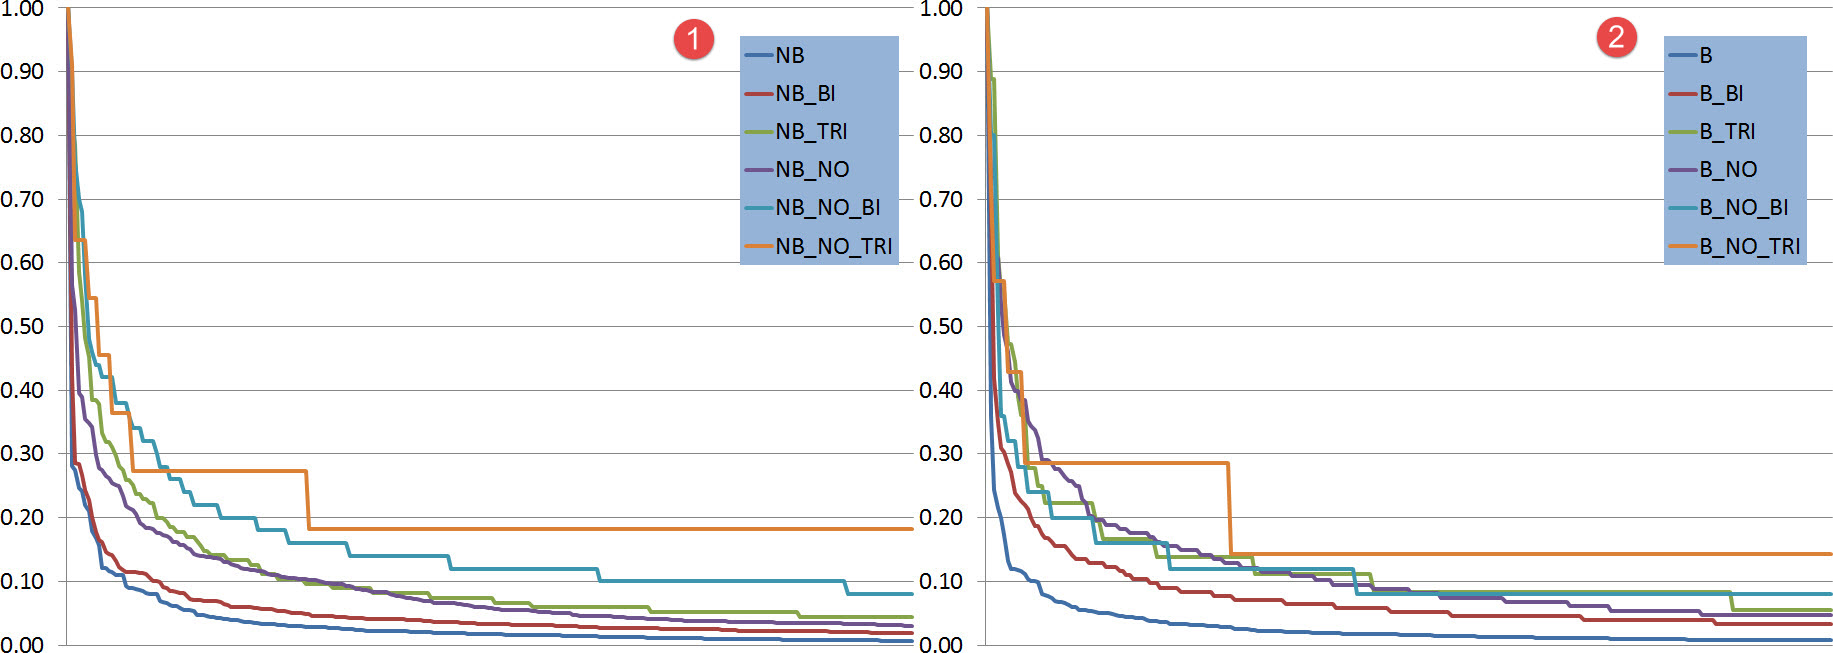
\includegraphics[width=1.0\textwidth]{Figures/Chapter4/word_frequencies_clean.jpg}
	\caption[Normalised distribution of word frequencies]{Graphs showing the normalised word distribution of the different token configurations examined}
	\label{fig:chapter4:word_frequencies_clean}
\end{figure}

\subsection{Data Visualisation Revisited}

Word clouds were also generated for bi-grams and tri-grams and the results can be seen in Figure \ref{fig:chapter4:bi-grams_wordclouds} and Figure \ref{fig:chapter4:trigram_wordclouds}. The many Eyes website was used once again with the same settings as before.

\begin{figure}[!htb]
	\centering
	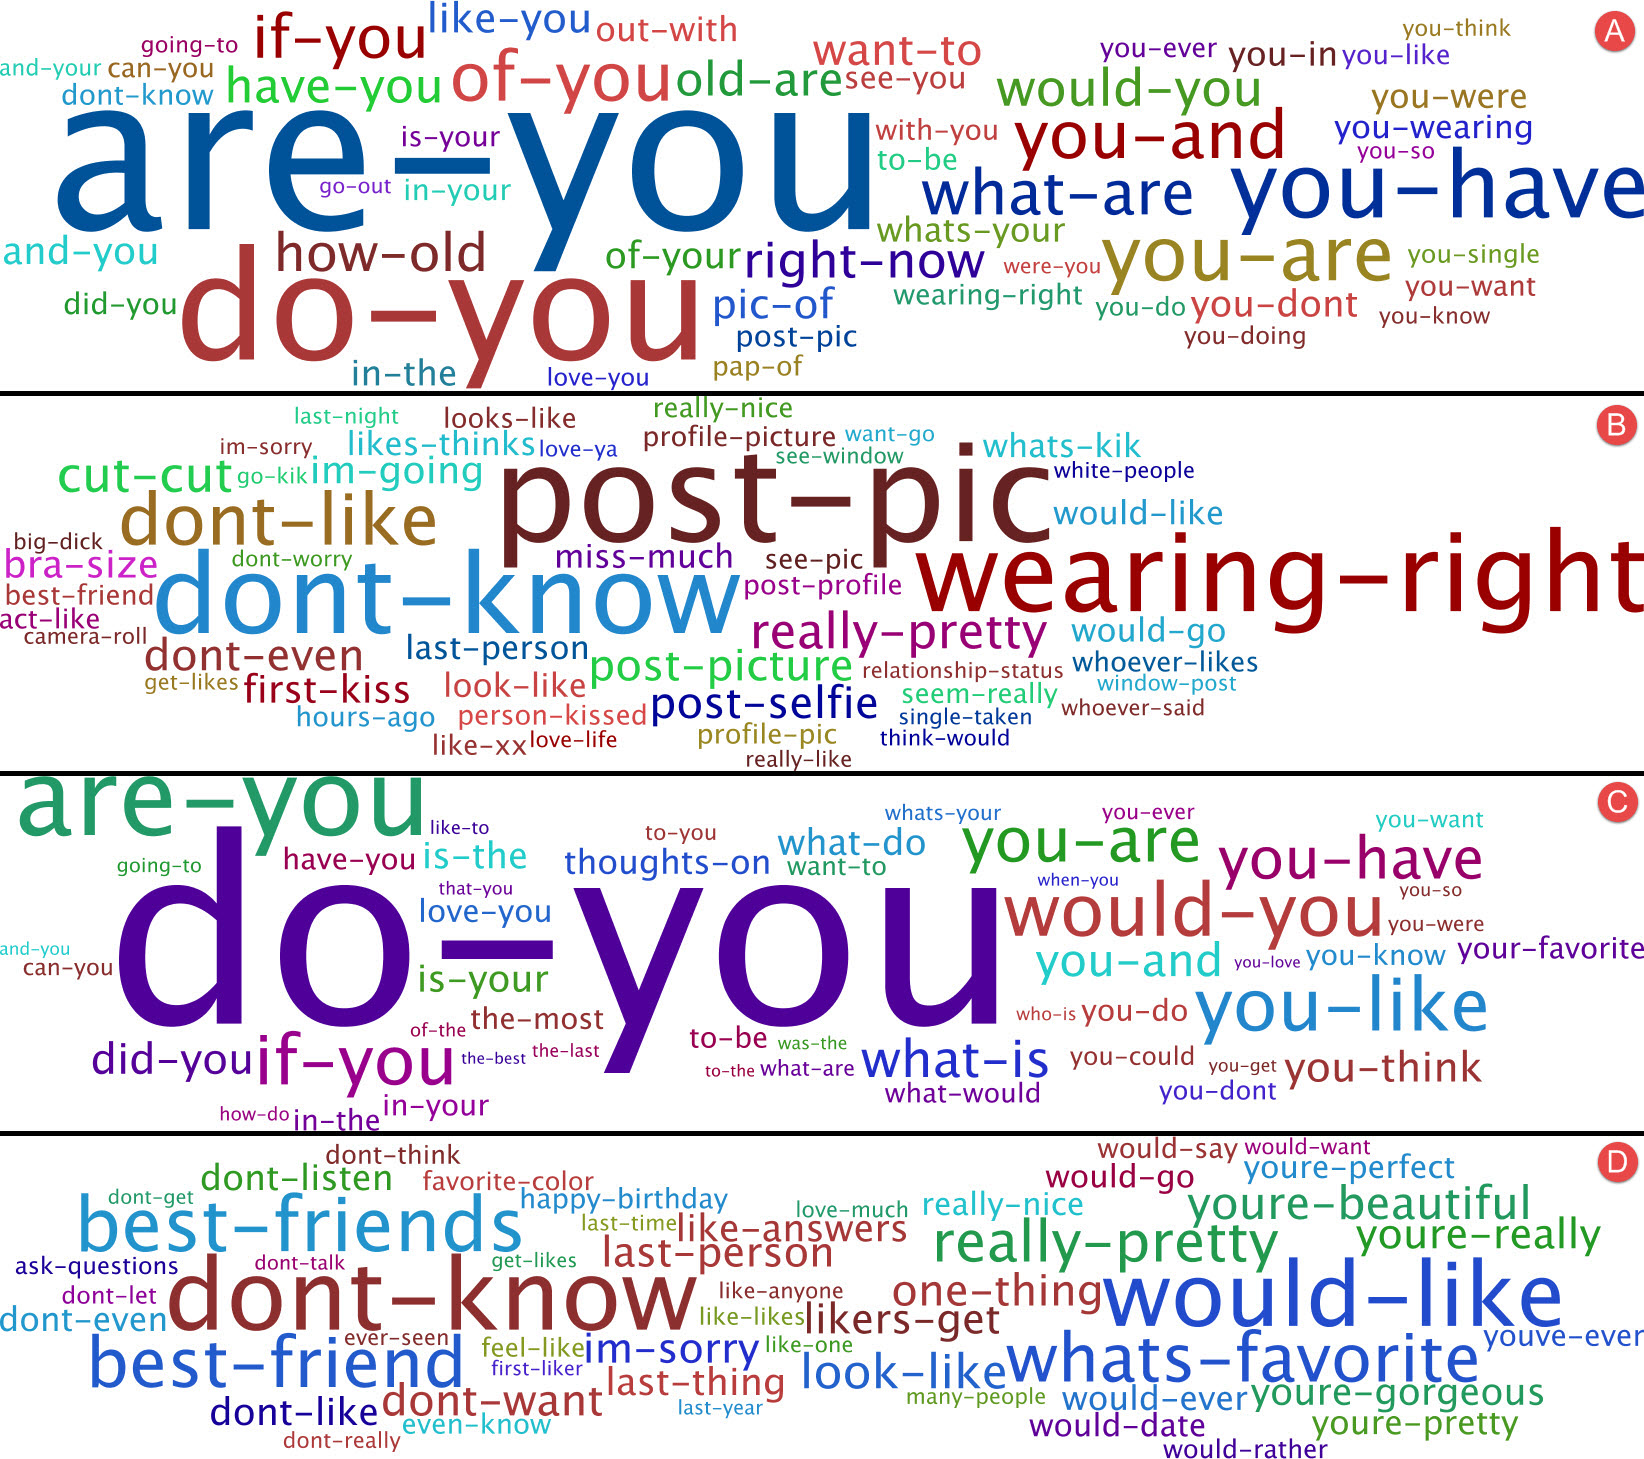
\includegraphics[width=1.0\textwidth]{Figures/Chapter4/bigram_clouds.jpg}
	\caption[Bi-gram word clouds]{Word clouds showing bullying bi-grams (a), bullying bi-grams with stop words removed (b), not bullying bi-grams (c) and not bullying bi-grams with stop words removed (d)}
	\label{fig:chapter4:bi-grams_wordclouds}
\end{figure}

\begin{figure}[!htb]
	\centering
	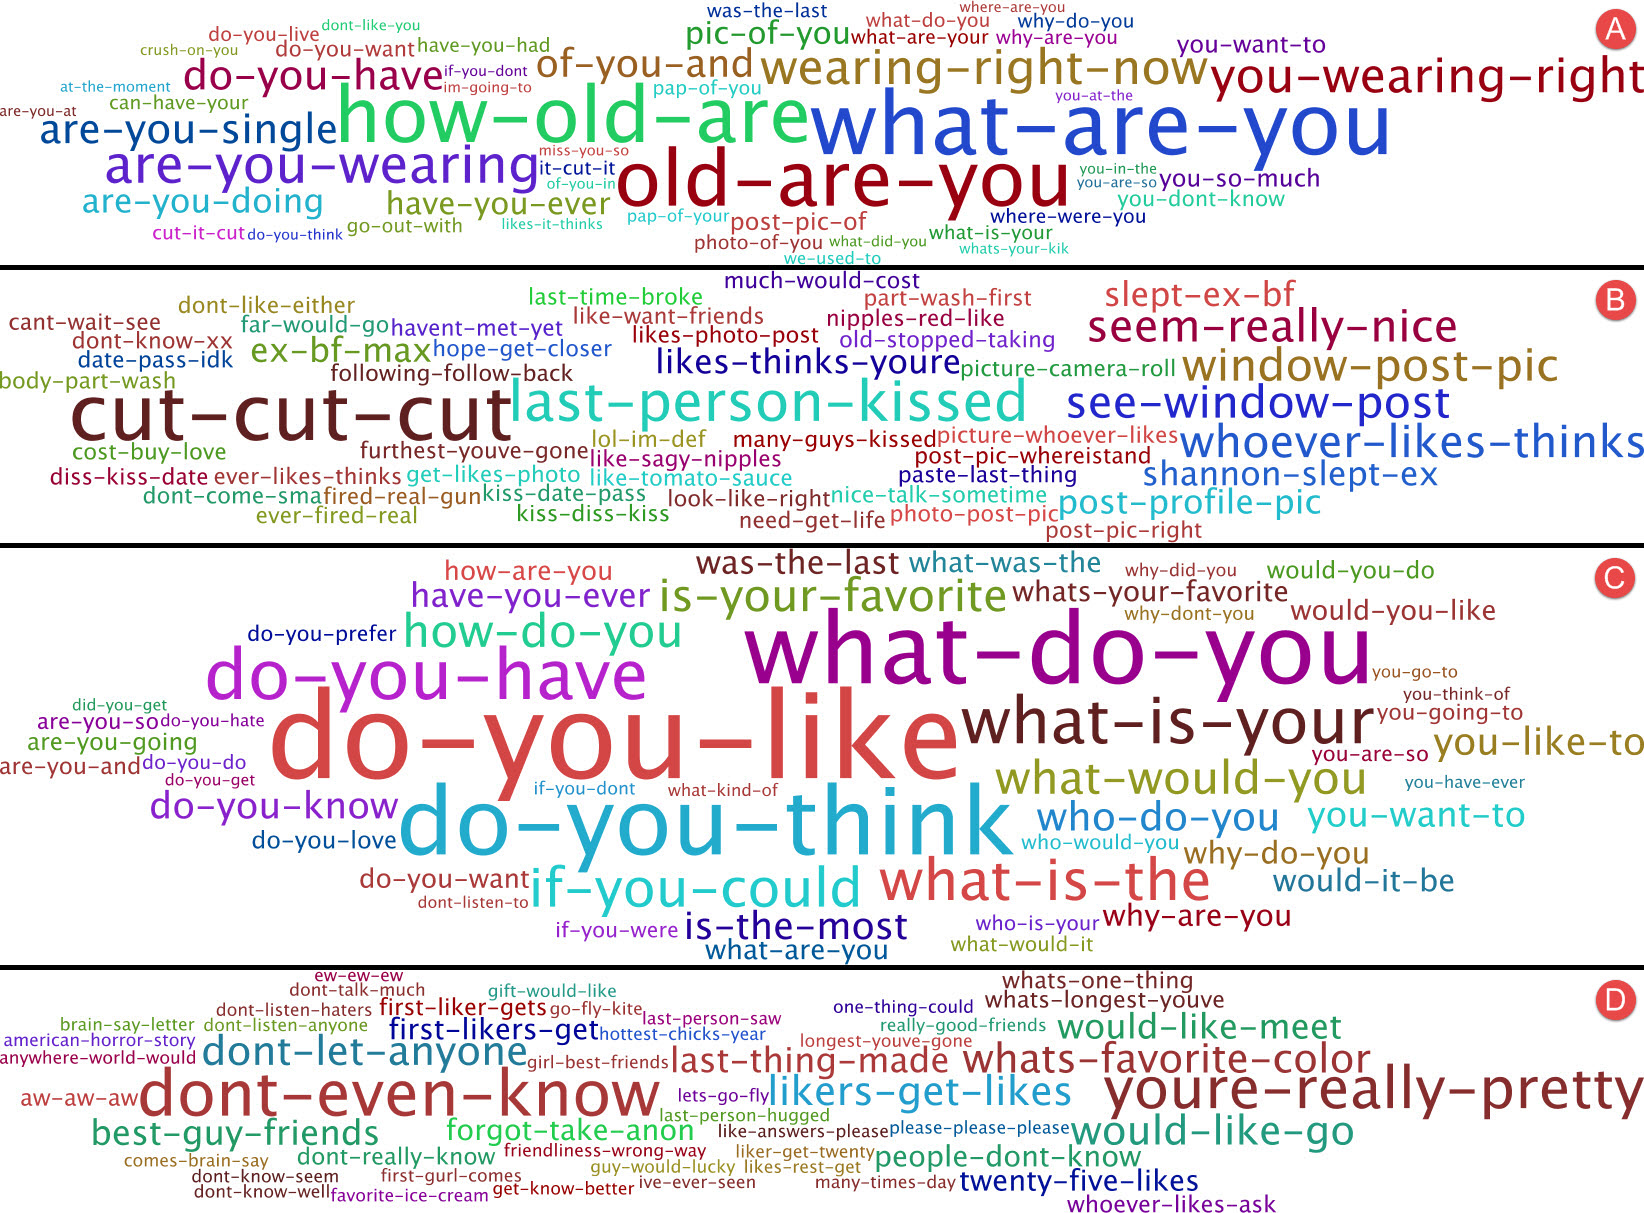
\includegraphics[width=1.0\textwidth]{Figures/Chapter4/trigram_clouds.jpg}
	\caption[Tri-gram word clouds]{Word clouds showing bullying tri-grams (a), bullying tri-grams with stop words removed (b), not bullying tri-grams (c) and not bullying tri-grams with stop words removed (d)}
	\label{fig:chapter4:trigram_wordclouds}
\end{figure}

As was seen with uni-grams the word clouds are dominated by stop words, especially the personal pronoun you. Looking at bi-grams first in Figure \ref{fig:chapter4:bi-grams_wordclouds}, the most frequently occurring bullying and not bullying tokens, \textit{``are\_you''} and \textit{``do\_you''}, are easily seen in section A and section C. Even after stop word removal, section B and section D, the bi-grams with the highest frequency occurrences are still clearly visible. Examining the tri-gram word clouds in Figure \ref{fig:chapter4:trigram_wordclouds} it is obvious that the tokens are now more evenly distributed. Even though the frequency of these bullying and not bullying tokens are more evenly distributed, when compared to uni-grams and bi-gram clouds, there are still a number prominent tokens. It is hoped that these tokens would be good predictors for both class types.



